\chapter{Physik}
\section{Kinematik}
\subsection{Geradlinige Bewegungen(Translation)}

\begin{shaded}
\begin{align}
	a(t)&=a_0=\frac{\diff v}{\diff t}=\dot{v}=\ddot{s} \\
	v(t)&=a_0\cdot t+v_0=\frac{\diff s}{\diff t}=\dot{s} \\
	s(t)&=\frac{1}{2}a_0\cdot t^2+v_0\cdot t+s_0
\end{align}
\end{shaded}

\subsection{Kreisbewegungen(Rotation)}

\begin{boxleft}
\bla{Winkelgrößen}
\des[\radian\per\second\tothe{2}]{\alpha}{Winkelbeschleunigung}\\
\des[\radian\per\second\tothe{1}]{\omega}{Winkelgeschwindigkeit}\\
\des[\radian]{\varphi}{Drehwinkel}
\end{boxleft}\begin{boxrightshaded}
\begin{align}
\alpha(t)&=\alpha_0=\frac{\diff \omega}{\diff t}=\dot{\omega}=\ddot{\varphi} \\
\omega(t)&=\alpha_0\cdot t+\omega_0=\frac{\diff \varphi}{\diff t}=\dot{\varphi} \\
\varphi(t)&=\frac{1}{2}\alpha_0\cdot t^2+\omega_0\cdot t+\varphi_0
\end{align}
\end{boxrightshaded}

\begin{boxleft}
\bla{Bahngrößen}
\des[\meter\per\second\tothe{2}]{a_t}{Beschleunigung(tan)}\\
\des[\meter\per\second\tothe{1}]{v}{Geschwindugkeit}\\
\des[\meter]{s}{Weg}
\end{boxleft}\begin{boxrightshaded}
\begin{align}
a_t(t)&=a_0=\frac{\diff v}{\diff t}=\dot{v}=\ddot{s} \\
v(t)&=a_0\cdot t+v_0=\frac{\diff s}{\diff t}=\dot{s} \\
s(t)&=\frac{1}{2}a_0\cdot t^2+v_0\cdot t+s_0
\end{align}
\end{boxrightshaded}

\begin{boxleft}\bla{Umrechnung}
Winkelgrößen $\Leftrightarrow$ Bahngrößen\\
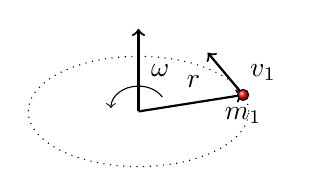
\begin{tikzpicture}[scale=.7]
  \draw[dotted] (1,.5) ellipse (2 and 1);
  \draw [<-,yscale=0.8] (.5,.7) arc (180:30:.5);

  \draw[->,thick] (1,.5)--(1,2); 
  \draw	(1,1.25)node[right=1pt]{$\vv{\omega}$};
     
\draw[->,thick] (1,.5) -- (2.9,.8);
\draw[<-,thick] (2.9,.8) +(130:1)--(2.9,.8)  ;
\draw (2,.7)node[above=1pt]{$\vv{r}$};
\draw	(2.8,1.2)node[right=1pt]{$\vv{v_1}$};
\draw (2.9,.8)node[below=1pt]{$m_1$};
\draw[shade,shading=ball,ball color=red] (2.9,.8) circle (.1);
 
\end{tikzpicture}
\end{boxleft}\begin{boxrightshaded}
\begin{align}
\vv{a_t}	&=\vv{\alpha} \times \vv{r}\\
a_t		&=\alpha\cdot r \qquad \alpha \perp r \\
\vv{\alpha}	&=\vv{r} \times \vv{a_t}\\
\vv{v}		&=\vv{\omega}\times\vv{r}\\
v		&=\omega\cdot r  \qquad \omega \perp r\\
\vv{\omega}	&=\vv{r} \times \vv{v}\\
s		&=\varphi\cdot r  
\end{align}
\end{boxrightshaded}

\begin{boxleft}\bla{Kreisfrequenz}
\des[\second]{T}{Periodendauer}\\
\des[\per\second]{n}{Drehzahl}\\
\des[\hertz]{f}{Frequenz}
\end{boxleft}\begin{boxrightshaded}
\begin{align}
\omega&=\frac{2\cdot\pi}{T}\\
&=2\cdot\pi\cdot n \\
&=2\cdot\pi\cdot f
\end{align}
\end{boxrightshaded}

\begin{boxleft}\bla{Radialbeschleunigung}
\des[\meter\per\second\tothe{2}]{a_r}{Radialbeschleunigung}
\end{boxleft}\begin{boxrightshaded}
\begin{align}
a_r&=\frac{v^2}{r}\\
&=v\cdot\omega\\
&=\omega^2\cdot r
\end{align}
\end{boxrightshaded}

\begin{boxleft}\bla{Umdrehungen}
\des{N}{Umdrehungen}
\end{boxleft}\begin{boxrightshaded}
\begin{align}
N	&=\frac{\omega_0\cdot t}{2\cdot \pi}+\frac{1}{2}\cdot\frac{\alpha}{2\cdot \pi}\cdot t^2\\
	&=n_0\cdot t+\frac{\alpha}{4\cdot\pi}\cdot t^2
\end{align}
\end{boxrightshaded}

\section{Dynamik}
\subsection{Geradlinig(Translation)}
\begin{boxleft}\bla{Kraft}
\des[\newton]{F}{Kraft}\\
\des[\kilo\gram]{m}{Masse}
\end{boxleft}\begin{boxrightshaded}
\begin{align}
\vv{F}&=m\cdot \vv{a}\\
\vv{F}_{\text{Tr}}&=-m\cdot \vv{a}
\end{align}
\end{boxrightshaded}

\begin{boxleft}\bla{Impuls}
\des[\kilo\gram\meter\per\second]{p}{Impuls}
\end{boxleft}\begin{boxrightshaded}
\begin{align}
\vv{p}&=m\cdot \vv{v}
\end{align}
\end{boxrightshaded}

\begin{boxleft}\bla{Kraftstoß}
\end{boxleft}\begin{boxrightshaded}
\begin{align}
\vv{F}&=\frac{\diff \vv{p}}{\diff t}=m\cdot\frac{\diff \vv{v}}{\diff t}+\vv{v}\cdot\frac{\diff m}{\diff t}\\
\Delta\vv{p}&=\vv{p}_2-\vv{p}_1=\int_{\vv{p}_2}^{\vv{p}_1}\diff p=\int_0^{t}\vv{F}\diff t
\end{align}
\end{boxrightshaded}

\begin{boxleft}\bla{Arbeit}
\des[\kilo\gram\meter\tothe{2}\per\second\tothe{2}]{W}{Arbeit}
\end{boxleft}\begin{boxrightshaded}
\begin{align}
W&=-\int_{\vv{s}_1}^{\vv{s}_2}\vv{F_{\text{Tr}}}\circ\diff \vv{s}\\
&=\int_{\vv{v}_0}^{\vv{v}_1}m\vv{v}\circ\diff \vv{v}=\frac{1}{2}m\left(v_1^2-v_0^2\right) 
\end{align}
\end{boxrightshaded}

\begin{boxleft}\bla{kin. Energie}
\des[\kilo\gram\meter\tothe{2}\per\second\tothe{2}]{E}{Energie}
\end{boxleft}\begin{boxrightshaded}
\begin{align}
E_{\text{kin}}=\frac{1}{2}mv^2
\end{align}
\end{boxrightshaded}


\begin{boxleft}\bla{Hubarbeit}
\des[\meter\per\second\tothe{2}]{g}{Fallbeschleunigung}
\end{boxleft}\begin{boxrightshaded}
\begin{align}
W_{\text{hub}}&=mgh
\end{align}
\end{boxrightshaded}

\begin{boxleft}\bla{Leistung}
\des[\kilo\gram\meter\tothe{2}\per\second\tothe{3}]{g}{Leistung}
\end{boxleft}\begin{boxrightshaded}
\begin{align}
P=\vv{F}\circ\vv{v}=\frac{\diff W}{\diff t}=\dot{W}
\end{align}
\end{boxrightshaded}


\subsection{Drehbewegung(Rotation)}

\begin{boxleft}\bla{Massenträgheitsmoment}
\des[\kilo\gram\meter\tothe{2}]{J}{Massenträgheitsmoment}
\end{boxleft}\begin{boxrightshaded}
\begin{align}
J=\int r^2 \diff m
\end{align}
\end{boxrightshaded}

\begin{boxleft}\bla{Drehimpuls}
\des[\kilo\gram\meter\tothe{2}\radian\per\second]{L}{Drehimpuls}
\end{boxleft}\begin{boxrightshaded}
\begin{align}
\vv{L}&=\vv{r}\times\vv{p} \\
&=J\cdot \vv{\omega}
\end{align}
\end{boxrightshaded}

\begin{boxleft}\bla{Drehmoment}
\des[\newton\meter]{M}{Drehmoment}
\end{boxleft}\begin{boxrightshaded}
\begin{align}
\vv{M}&=\vv{r}\times\vv{F}=J\vv{\alpha}=\dot{\vv{L}}
\end{align}
\end{boxrightshaded}

\begin{boxleft}\bla{kinetische Energie}
\end{boxleft}\begin{boxrightshaded}
\begin{align}
E_{kin}=\frac{1}{2}J\omega^2
\end{align}
\end{boxrightshaded}

\begin{boxleft}\bla{Arbeit}
\end{boxleft}\begin{boxrightshaded}
\begin{align}
W	&=\int_{\varphi_0}^{\varphi_1}\vv{M}\circ\vv{e_\omega}\diff \varphi=\int_{\vv{\omega}_0}^{\vv{\omega}_1}J\vv{\omega}\diff\vv{\omega}\\
&=\frac{1}{2}J\left(\omega_1^2-\omega_0^2\right)
\end{align}
\end{boxrightshaded}


\begin{boxleft}\bla{Leistung}
\end{boxleft}\begin{boxrightshaded}
\begin{align}
P=\vv{M}\circ\vv{\omega}
\end{align}
\end{boxrightshaded}

\begin{boxleft}\bla{Zentripedalkraft}
\end{boxleft}\begin{boxrightshaded}
\begin{align}
F_{zp}&=-m\cdot\omega^2\cdot r\\
&=-m\cdot v^2\cdot \frac{\vv{e_r}}{r}
\end{align}
\end{boxrightshaded}

\subsection{Schiefe Ebene}

\begin{boxleft}\bla{Kräfte}
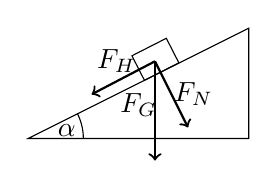
\begin{tikzpicture}[scale=.7]
  \draw (0,0) -- (4,0) -- (4,2)-- cycle;
  \draw[yshift=30,xshift=60,rotate=27] (0,0) -- (0,.5) -- (.7,.5) -- (.7,0) --cycle;
    
  \draw (1,0) arc (0:27:1);
  \draw (.7,0.15)node{$\alpha$};

  \draw[thick,->] (2.3,1.4)--(2.3,-.4);
  \draw[thick,->] (2.3,1.4)--(1.15,.8);
  \draw[thick,->] (2.3,1.4)--(2.9,.2);

  \draw (1.6,1.4)node{$\vv{F}_H$};
  \draw (3,0.8)node{$\vv{F}_N$};
  \draw (2,0.6)node{$\vv{F}_G$};
\end{tikzpicture}
\end{boxleft}\begin{boxrightshaded}
\begin{align}
\vv{F}_N&=\vv{F}_G\cos\alpha\\
\vv{F}_H&=\vv{F}_G\sin\alpha
\end{align}
\end{boxrightshaded}

\subsection{Reibung}

\begin{boxleft}\bla{Reibungskräfte}
\des[\newton]{F_N}{Normalkraft}\\
\des[\newton]{F_R}{Reibungskraft}\\
\des{\mu}{Reibungskoeffizient}
\end{boxleft}\begin{boxrightshaded}
\begin{align}
F_R=\mu\cdot F_N
\end{align}
\end{boxrightshaded}

\begin{boxleft}\bla{Rollreibung}
\des[\newton]{F_N}{Normalkraft}\\
\des{f}{Rollreibungstahl}\\
\des{M}{Drehmoment}\\
\des[\meter]{r}{Radius}
\end{boxleft}\begin{boxrightshaded}
\begin{align}
M&=f\cdot F_N\\
F_R&=\frac{f}{r}\cdot F_N
\end{align}
\end{boxrightshaded}

\subsection{Feder}

\begin{boxleft}\bla{Hookesches Gesetz}
\des[\newton\per\meter]{k}{Federkonstante}\\
\des[\newton\meter\per\radian]{D}{Winkelrichtgröße}
\end{boxleft}\begin{boxrightshaded}
\begin{align}
F&=-kx\\
M&=D\varphi
\end{align}
\end{boxrightshaded}

\begin{boxleft}\bla{Spannungsenergie}
\end{boxleft}\begin{boxrightshaded}
\begin{align}
W	&=\int_{x_\text{min}}^{x_\text{max}}F\diff x=\int_{x_\text{min}}^{x_\text{max}}kx\diff x\\
	&=\frac{1}{2}\cdot k\cdot \left(x_{\text{max}}^2-x_{\text{min}}^2\right)
\end{align}
\end{boxrightshaded}

\subsection{Elastischer Stoß}

\begin{boxleft}\bla{Energieerhaltung}
\end{boxleft}\begin{boxrightshaded}
\begin{align}
\text{Energie vor den Stoß} &= \text{Energie nach den Stoß}\nonumber\\
\sum E_{\text{kin}}&=\sum E_{\text{kin}}'
\end{align}
\end{boxrightshaded}

\begin{boxleft}\bla{Impulserhaltung}
\end{boxleft}\begin{boxrightshaded}
\begin{align}
\text{Impuls vor den Stoß} &= \text{Impuls nach den Stoß}\nonumber\\
\sum m\vv{v}&= \sum m\vv{v}'
\end{align}
\end{boxrightshaded}

\begin{boxleft}\bla{Zentraler, elastischer Stoß}
\destext{(Energie und Impuls)}
\end{boxleft}\begin{boxrightshaded}
\begin{align}
\frac{1}{2}m_1v_1^2+\frac{1}{2}m_2v_2^2&=\frac{1}{2}m_1v_1'^2+\frac{1}{2}m_2v_2'^2\\
m_1v_1+m_2v_2&=m_1v_1'+m_2v_2'
\end{align}
\end{boxrightshaded}

\begin{boxleft}\bla{Zentraler, elastischer Stoß}
\destext{(Geschwindigkeit nach dem Stoß)}
\end{boxleft}\begin{boxrightshaded}
\begin{align}
v_2'&=\frac{2m_1}{m_1+m_2}v_1+\frac{m_2-m_1}{m_1+m_2}v_2\\
v_1'&=\frac{2m_2}{m_1+m_2}v_2+\frac{m_1-m_2}{m_1+m_2}v_1
\end{align}
\end{boxrightshaded}

\subsection{Unelastischer Stoß}

\begin{boxleft}\bla{Energieerhaltung}
\end{boxleft}\begin{boxrightshaded}
\begin{align}
\text{Energie vor den Stoß} &= \text{Energie nach den Stoß}+\text{Arbeit}\nonumber\\
\sum E_{\text{kin}}&=\sum E_{\text{kin}}'+\Delta W
\end{align}
\end{boxrightshaded}

\begin{boxleft}\bla{Impulserhaltung}
\end{boxleft}\begin{boxrightshaded}
\begin{align}
\text{Impuls vor den Stoß} &= \text{Impuls nach den Stoß}\nonumber\\
\sum m\vv{v}&= \sum m\vv{v}'
\end{align}
\end{boxrightshaded}

\begin{boxleft}\bla{Total unelastischer Stoß}
\destext{(Energie und Impuls)}
\end{boxleft}\begin{boxrightshaded}
\begin{align}
\frac{1}{2}m_1v_1^2+\frac{1}{2}m_2v_2^2&=\frac{1}{2}\left(m_1+m_2\right)v'^2+\Delta W\\
m_1v_1+m_2v_2&=\left(m_1+m_2\right)v'
\end{align}
\end{boxrightshaded}

\begin{boxleft}\bla{Total unelastischer Stoß}
\destext{(Geschwindigkeit nach dem Stoß)}
\end{boxleft}\begin{boxrightshaded}
\begin{align}
v'		&=\frac{m_1v_1+m_2v2}{m_1+m_2}
\end{align}
\end{boxrightshaded}

\begin{boxleft}\bla{Total unelastischer Stoß}
\destext{(Energieverlust)}
\end{boxleft}\begin{boxrightshaded}
\begin{align}
\Delta W	&=\frac{m_1\cdot m_2}{2\left(m_1+m_2\right)}\left(v_1-v_2\right)^2
\end{align}
\end{boxrightshaded}
\subsection{Drehimpulse}

\begin{boxleft}\bla{Drehimpulserhaltungssatz}
\end{boxleft}\begin{boxrightshaded}
\begin{align}
\text{Drehinpuls zur Zeit 1} &= \text{Drehimpuls zur Zeit 2}\\
\sum \vv{L}&=\sum \vv{L}'
\end{align}
\end{boxrightshaded}

\begin{boxleft}\bla{Kupplung Zweier Drehkörper}
\destext{(Winkelgeschwindigkeit nach dem Kuppeln und Energieverlust)}
\end{boxleft}\begin{boxrightshaded}
\begin{align}
\vv{\omega}'&=\frac{J_0\vv{\omega_0}+J_1\vv{\omega_1}}{J_1+J_2}\\
W&=\frac{J_0\cdot J_1}{2\left(J_0+J_1\right)}\left(\omega_0-\omega_1\right)^2
\end{align}
\end{boxrightshaded}


\subsection{Rotierendes Bezugssystem}

\begin{boxleft}\bla{Zentrifugalkraft}
\end{boxleft}\begin{boxrightshaded}
\begin{align}
\vv{F}_Z&=F_r\cdot \vv{e}_r=-m\vv{\omega}\times\left(\vv{\omega}\times\vv{r}\right)=-m\vv{\omega}\times\vv{v}\\
  F_Z&=-m\frac{v^2}{r}=-m\omega^2 r
\end{align}
\end{boxrightshaded}

\begin{boxleft}\bla{Corioliskraft}
\end{boxleft}\begin{boxrightshaded}
\begin{align}
\vv{F}_C&=-2m\vv{\omega}\times\vv{v}
\end{align}
\end{boxrightshaded}

\section{Schwerpunkt}

\begin{boxleft}\bla{Schwerpunkt mehrere Punktmassen}
\end{boxleft}\begin{boxrightshaded}
\begin{align}
\vv{r}_{\text{Sp}}=\frac{\sum\vv{r}_i m_i}{\sum\ m_i}
\end{align}
\end{boxrightshaded}

\begin{boxleft}\bla{Allgemein Schwerpunkt}
\end{boxleft}\begin{boxrightshaded}
\begin{align}
\vv{r}_{\text{Sp}}=\frac{\int \vv{r}\diff m}{\int \diff m}
\end{align}
\end{boxrightshaded}

\begin{boxleft}\bla{Schwerpunkt (Kartesische)}
\des[\kilo\gram\per\meter\tothe{3}]{\rho}{Dichte}
\end{boxleft}\begin{boxrightshaded}
\begin{align}
x_{\text{Sp}}&=\frac{\int_z\int_y\int_x x\rho \diff x \diff y \diff z }{\int_z\int_y\int_x \rho \diff x \diff y \diff z }\\
y_{\text{Sp}}&=\frac{\int_z\int_y\int_x y\rho \diff x \diff y \diff z }{\int_z\int_y\int_x \rho \diff x \diff y \diff z }\\
z_{\text{Sp}}&=\frac{\int_z\int_y\int_x z\rho \diff x \diff y \diff z }{\int_z\int_y\int_x \rho \diff x \diff y \diff z }
\end{align}
\end{boxrightshaded}

\begin{boxleft}\bla{Schwerpunkt (Zylinder)}
\end{boxleft}\begin{boxrightshaded}
\begin{align}
r_{\text{Sp}}&=\frac{\int_z\int_\varphi\int_r r^2\rho \diff r \diff \varphi \diff z }{\int_z\int_\varphi\int_r r\rho \diff r \diff \varphi \diff z }\\
\varphi_{\text{Sp}}&=\frac{\int_z\int_\varphi\int_r \varphi r\rho \diff r \diff \varphi \diff z }{\int_z\int_\varphi\int_r r\rho \diff r \diff \varphi \diff z }\\
z_{\text{Sp}}&=\frac{\int_z\int_\varphi\int_r z r\rho \diff r \diff \varphi \diff z }{\int_z\int_\varphi\int_r r\rho \diff r \diff \varphi \diff z }\\
x&=r\cos{\varphi}\\
y&=r\sin{\varphi}\\
z&=z
\end{align}
\end{boxrightshaded}

\section{Trägheitsmoment}


\begin{boxleft}\bla{Allgemein}
\des[\kilo\gram\per\meter\tothe{3}]{\rho}{Dichte}\\
\des[\kilo\gram\meter\tothe{2}]{J}{Massenträgheitsmoment}
\end{boxleft}\begin{boxrightshaded}
\begin{align}
J&=\sum m_i r_i^2\\
J&=\int_m r^2 \diff m \\
J&=\int_z\int_\varphi\int_r r^3\rho \diff r \diff \varphi \diff z 
\end{align}
\end{boxrightshaded}

\begin{boxleft}\bla{Satz von Steiner}
\des[\kilo\gram\meter\tothe{2}]{J_s}{Mtm am der alten Achse}\\
\des[\kilo\gram\meter\tothe{2}]{J_x}{Mtm am der neuen Achse $(J_x\parallel J_s)$)}
\end{boxleft}\begin{boxrightshaded}
\begin{align}
J_x&=mr^2+J_s
\end{align}
\end{boxrightshaded}

\begin{boxleft}\bla{Trägheitsmoment Kugel}
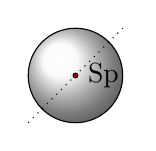
\begin{tikzpicture}[scale=.3]
  \draw[ball color=gray!5] (2,2) circle (2);
  \draw[fill=red] (2,2) circle (.1);
  \draw[dotted](0,0)--(4,4);
  \draw(2,2)node[right=1pt]{Sp};
\end{tikzpicture}\end{boxleft}\begin{boxrightshaded}
\begin{align}
J_\text{Sp}&=\frac{2}{5}mr^2
\end{align}
\end{boxrightshaded}

\begin{boxleft}\bla{Trägheitsmoment Zylinder}
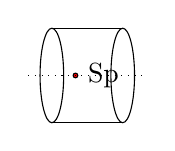
\begin{tikzpicture}[scale=.3]
  \draw (1,2) ellipse (.5 and 2);
  \draw (1,4) -- (4,4);
  \draw (1,0) -- (4,0);
  \draw (4,2) ellipse (.5 and 2);
  \draw[fill=red] (2,2) circle (.1);
  \draw[dotted](0,2)--(5,2);
  \draw(2,2)node[right=1pt]{Sp};
\end{tikzpicture}\end{boxleft}\begin{boxrightshaded}
\begin{align}
J_\text{Sp}&=\frac{1}{2}mr^2
\end{align}
\end{boxrightshaded}

\begin{boxleft}\bla{Trägheitsmoment Kreisring}
\end{boxleft}\begin{boxrightshaded}
\begin{align}
J_\text{Sp}&=mr^2
\end{align}
\end{boxrightshaded}

\begin{boxleft}\bla{Trägheitsmoment Stab}
\end{boxleft}\begin{boxrightshaded}
\begin{align}
J_\text{Sp}=\frac{1}{12}ml^2
\end{align}
\end{boxrightshaded}

\section{Elastizitätslehre}

\begin{boxleft}\bla{Spannung}
\des[\newton\per\meter\tothe{2}]{\sigma}{Normalspannung}\\
\des[\newton\per\meter\tothe{2}]{\tau}{Schubspannung}\\
\des[\newton\per\meter\tothe{2}]{E}{Elastizitätsmodul}\\
\des[\newton]{F_n}{Normalkraft $(\vv{F} \parallel \vv{A}$}\\
\des{\varepsilon}{Dehnung}
\end{boxleft}\begin{boxrightshaded}
\begin{align}
\vv{\sigma}&=\frac{\diff\vv{F}_n}{\diff A}\\
\sigma&=E \varepsilon=E\frac{\Delta l}{l}\\
\vv{\tau}&= \frac{\diff\vv{F}_t}{\diff A}
\end{align}
\end{boxrightshaded}

\begin{boxleft}\bla{Schubmodul}
\des[\newton\per\meter\tothe{2}]{G}{Schubmodul}\\
\des[\radian]{\varphi}{Scherwinkel}
\end{boxleft}\begin{boxrightshaded}
\begin{align}
G&=\frac{\tau}{\varphi}
\end{align}
\end{boxrightshaded}

\begin{boxleft}\bla{Drillung}
\des[\radian\per\meter]{\psi}{Drillung}\\
\des[\radian]{\varphi}{Torisionswinkel}\\
\des[\meter]{l}{Länge des Drehkörpers}\\
\des[\meter\tothe{3}]{W_t}{Wiederstandsmoment}
\end{boxleft}\begin{boxrightshaded}
\begin{align}
\psi&=\frac{\diff \varphi}{\diff l}=\frac{W_t}{G\cdot J_p}\tau=\frac{M_t}{G\cdot J_p}
\end{align}
\end{boxrightshaded}

\begin{boxleft}\bla{Polares Fläschenmoment}
\des[\meter\tothe{4}]{J_p}{Polares Fläschenmoment}
\end{boxleft}\begin{boxrightshaded}
\begin{align}
J_p&=\int r^2\diff A=\int_\varphi\int_r r^3\diff r \diff \varphi 
\end{align}
\end{boxrightshaded}

\begin{boxleft}\bla{Verformungsarbeit}
\end{boxleft}\begin{boxrightshaded}
\begin{align}
W&=V\int \sigma(\varepsilon) \diff \varepsilon 
\end{align}
\end{boxrightshaded}

\section{Schwingungen}


\begin{boxleft}\bla{Harmonische Schwingung}
\des{A}{Amplitude}\\
\des[\radian\per\second]{\omega}{Kreisfrequenz}\\
\des[\radian]{\varphi}{phasenverschiebung}
\end{boxleft}\begin{boxrightshaded}
\begin{align}
u(t)=A\cos(\omega t+\varphi_0)
\end{align}
\end{boxrightshaded}

\subsection{Ungedämpfte Schwingungen}

\begin{boxleft}\bla{Federpendel}
\des[\meter]{\hat{x}}{Amplitude}\\
\des[\kilo\gram\per\second\tothe{2}]{k}{Federkonstante}\\
\des[\radian\per\second]{\omega}{Eigenfrequenz}
\end{boxleft}\begin{boxrightshaded}
\begin{align}
\ddot{x}&=-\frac{k}{m}x\\
x(t)&=\hat{x}\cos(\omega_0 t+\varphi_0)\\
\dot{x}(t)&=-\hat{x}\omega\sin(\omega_0 t+\varphi_0)\\
\ddot{x}(t)&=-\hat{x}\omega^2\cos(\omega_0 t+\varphi_0)\\
\omega&=\sqrt{\frac{k}{m}}\\
f&=\frac{1}{2\pi}\sqrt{\frac{k}{m}}\\
T&=2\pi\sqrt{\frac{m}{k}}
\end{align}
\end{boxrightshaded}

\begin{boxleft}\bla{Mathematisches Pendel}
\des[\radian]{\varphi}{Auslenkwinkel}\\
\des[\radian]{\hat{\varphi}}{Amplitude}\\
\des[\meter\per\second\tothe{2}]{g}{Fallbeschleunigung}\\
\des[\radian\per\second]{\omega}{Eigenfrequenz}\\
\des[\meter]{l}{Pendellänge}
\end{boxleft}\begin{boxrightshaded}
\begin{align}
\ddot{\varphi}&=-\frac{g}{l}\varphi\\
\varphi(t)&=\hat{\varphi}\cos(\omega_0 t+\varphi_0)\\
\dot{\varphi}(t)&=-\hat{\varphi}\omega\sin(\omega_0 t+\varphi_0)\\
\ddot{\varphi}(t)&=-\hat{\varphi}\omega^2\cos(\omega_0 t+\varphi_0)\\
\omega&=\sqrt{\frac{g}{l}}\\
f&=\frac{1}{2\pi}\sqrt{\frac{g}{l}}\\
T&=2\pi\sqrt{\frac{l}{g}}
\end{align}
\end{boxrightshaded}

\begin{boxleft}\bla{Physikalisches Pendel}
\des[\radian]{\varphi}{Auslenkwinkel}\\
\des[\radian]{\hat{\varphi}}{Amplitude}\\
\des[\meter\per\second\tothe{2}]{g}{Fallbeschleunigung}\\
\des[\radian\per\second]{\omega}{Eigenfrequenz}\\
\des[\meter]{l}{Abstand Drehachse A zum SP}\\
\des[\kilo\gram\meter\tothe{2}]{J_A}{Trägheitsmoment um Achse A}
\end{boxleft}\begin{boxrightshaded}
\begin{align}
\ddot{\varphi}&=-\frac{lmg}{J_A}\varphi\\
\varphi(t)&=\hat{\varphi}\cos(\omega_0 t+\varphi_0)\\
\dot{\varphi}(t)&=-\hat{\varphi}\omega\sin(\omega_0 t+\varphi_0)\\
\ddot{\varphi}(t)&=-\hat{\varphi}\omega^2\cos(\omega_0 t+\varphi_0)\\
\omega&=\sqrt{\frac{mgl}{J_A}}\\
f&=\frac{1}{2\pi}\sqrt{\frac{mgl}{J_A}}\\
T&=2\pi\sqrt{\frac{J_A}{mgl}}
\end{align}
\end{boxrightshaded}

\begin{boxleft}\bla{Torisionsschwingung}
\des[\radian]{\varphi}{Torisionswinkel}\\
\des[\radian]{\hat{\varphi}}{Amplitude}\\
\des[\radian\per\second]{\omega}{Eigenfrequenz}\\
\des[\radian\per\second]{D}{Winkelrichtgröße}\\
\des[\kilo\gram\meter\tothe{2}]{J_A}{Trägheitsmoment um Achse A}
\end{boxleft}\begin{boxrightshaded}
\begin{align}
\ddot{\varphi}&=-\frac{D}{J_A}\varphi\\
\varphi(t)&=\hat{\varphi}\cos(\omega_0 t+\varphi_0)\\
\dot{\varphi}(t)&=-\hat{\varphi}\omega\sin(\omega_0 t+\varphi_0)\\
\ddot{\varphi}(t)&=-\hat{\varphi}\omega^2\cos(\omega_0 t+\varphi_0)\\
\omega&=\sqrt{\frac{D}{J_A}}\\
f&=\frac{1}{2\pi}\sqrt{\frac{D}{J_A}}\\
T&=2\pi\sqrt{\frac{J_A}{D}}
\end{align}
\end{boxrightshaded}

\begin{boxleft}\bla{Flüssigkeitspendel}
\des[\meter]{y}{Auslenkung}\\
\des[\meter]{\hat{y}}{Amplitude}\\
\des[\radian\per\second]{\omega}{Eigenfrequenz}\\
\des[\kilo\gram\per\meter\tothe{2}]{\rho}{Dichte der Flüssigkeit}\\
\des[\meter]{l}{Länge der Flüssigkeitsseule}\\
\des[\meter\tothe{2}]{A}{Querschnittsfläche}
\end{boxleft}\begin{boxrightshaded}
\begin{align}
\ddot{y}&=-\frac{2A\rho g}{m}y\\
\varphi(t)&=\hat{y}\cos(\omega_0 t+\varphi_0)\\
\dot{\varphi}(t)&=-\hat{y}\omega\sin(\omega_0 t+\varphi_0)\\
\ddot{\varphi}(t)&=-\hat{y}\omega^2\cos(\omega_0 t+\varphi_0)\\
\omega&=\sqrt{\frac{2A\rho g}{m}}=\sqrt{\frac{2g}{l}}\\
f&=\frac{1}{2\pi}\sqrt{\frac{2g}{l}}\\
T&=2\pi\sqrt{\frac{l}{2g}}
\end{align}
\end{boxrightshaded}

\begin{boxleft}\bla{Elektrischer Schwingkreis}
\des[\ampere\second]{q}{Ladung}\\
\des[\ampere\second]{\hat{q}}{Amplitude, max. Ladung Kondensator}\\
\des[\volt\second\per\ampere]{L}{Induktivität}\\
\des[\ampere\second\per\volt]{C}{Kapazität}
\end{boxleft}\begin{boxrightshaded}
\begin{align}
0&=L\ddot{Q}+\frac{Q}{C}\\
q(t)&=\hat{Q}\cos(\omega_0 t+\varphi_0)\\
\dot{q}(t)&=-\hat{Q}\omega\sin(\omega_0 t+\varphi_0)\\
\ddot{q}(t)&=-\hat{Q}\omega^2\cos(\omega_0 t+\varphi_0)\\
\omega&=\sqrt{\frac{1}{LC}}\\
f&=\frac{1}{2\pi}\sqrt{\frac{1}{LC}}\\
T&=2\pi\sqrt{\frac{1}{LC}}
\end{align}
\end{boxrightshaded}

\subsection{Gedämpfte Schwingungen}

\begin{boxleft}\bla{Schwingungsgleichung mit Reibung}
\des[\kilo\gram\per\second\tothe{2}]{k}{Richtgröße}\\
\des[\newton]{F_R}{Reibungskraft}\\
\des[\metre]{x}{Auslenkung}
\end{boxleft}\begin{boxrightshaded}
\begin{align}
m\ddot{x}=-kx+F_R
\end{align}
\end{boxrightshaded}

\begin{boxleft}\bla{Coulomb-Reibung}
\des[\kilo\gram\per\second\tothe{2}]{k}{Richtgröße}\\
\des[\newton]{F_N}{Normalkraft}\\
\des[\newton]{F_R}{Reibungskraft}\\
\des{\mu}{Reibungskoeffizient}\\
\des[\metre\per\second]{\dot{x}}{Geschwindigkeit}
\end{boxleft}\begin{boxrightshaded}
\begin{align}
F_R&=-\operatorname{sgn}({\dot{x}})\mu F_N\\
0&=m\ddot{x}+kx+\operatorname{sgn}({\dot{x}})\mu F_N\\
\operatorname{sgn}({\dot{x}})&=
\begin{dcases*}
  -1&$\dot{x}<0$\\
\phantom{+}0& $\dot{x}=0$\\
  +1&$\dot{x}>0$
\end{dcases*}
\end{align}
\end{boxrightshaded}

\begin{boxleft}\bla{Gleitreibung(Nicht Behandelt)}
\des[\kilo\gram\per\second\tothe{2}]{k}{Richtgröße}\\
\des[\newton]{F_N}{Normalkraft}\\
\des{\mu}{Reibungskoeffizient}\\
\des[\meter]{\hat{x}_0}{Start Amplitude}\\
\des[\meter]{\hat{x}_1}{End Amplitude}
\end{boxleft}\begin{boxrightshaded}
\begin{align}
x(t)&=-(\hat{x}_0-\hat{x}_1)\cos(\omega t)-\hat{x}_1\qquad 0\leq t\leq \frac{T}{2}\\
x(t)&=-(\hat{x}_0-3\hat{x}_1)\cos(\omega t)+\hat{x}_1\qquad \frac{T}{2}\leq t\leq T\\
\hat{x}_1&=\frac{\mu F_N}{k}
\end{align}
\end{boxrightshaded}

\begin{boxleft}\bla{Viskose Reibung}
\des[\kilo\gram\per\second\tothe{2}]{k}{Richtgröße}\\
\des[\meter]{\hat{x}}{Amplitude}\\
\des[\radian\per\second]{\omega}{Eigenfrequenz}\\
\des[\per\second]{\delta}{Abklingkoeffizient}\\
\des[\kilo\gram\per\second]{b}{Dämpfungskonstante}\\
\des{D}{Dämpfungsgrad}\\
\des[\radian\per\second]{\omega_D}{Gedämpfte Kreisfrequenz}\\
\des[\kilo\gram\per\second]{\delta}{logarithmischen Dekrement}\\
\des{d}{Verlustfaktor}\\
\des{Q}{Güte}
\end{boxleft}\begin{boxrightshaded}
\begin{align}
0&=m\ddot{x}+b\dot{x}+kx\\
x(t)&=\hat{x}e^{-\delta t}e^{\pm j\sqrt{\omega_0^2-\delta^2}t}\\
x(t)&=\hat{x}e^{-\delta t}e^{\pm j\omega_0\sqrt{1-D^2}t}\\
\delta&=\frac{b}{2m}\\
D&=\frac{\delta}{\omega_0}\\
D&=\frac{b}{2}\frac{1}{\sqrt{mk}}\\
\omega_0&=\sqrt{\frac{k}{m}}\\
\Lambda&=\ln\left(\frac{x(t)}{x(t+T)}\right)\\
\Lambda&=\delta T\\
\omega_D&=\sqrt{\frac{k}{m}-\left(\frac{b}{2m}\right)^2}\\
d&=2D\\
Q&=\frac{1}{d}
\end{align}
\end{boxrightshaded}

\begin{boxleft}\bla{Viskose Reibung}
\destext{Schwingfall.$\delta<\omega_0$}
\end{boxleft}\begin{boxrightshaded}
\begin{align}
x(t)&=\hat{x}e^{-\delta t}\cos(\sqrt{\omega_0^2-\delta^2}t+\varphi)
\end{align}
\end{boxrightshaded}

\begin{boxleft}\bla{Viskose Reibung}
\destext{Aperiodischer Grenzfall $\delta=\omega_0$}
\end{boxleft}\begin{boxrightshaded}
\begin{align}
x(t)&=\hat{x}e^{-\delta t}(1-\delta t)
\end{align}
\end{boxrightshaded}

\begin{boxleft}\bla{Viskose Reibung}
\destext{Kriechfall $\delta>\omega_0$}
\end{boxleft}\begin{boxrightshaded}
\begin{align}
x(t)&=\hat{x}e^{-\delta t}e^{\pm j\sqrt{\omega_0^2-\delta^2}t}
\end{align}
\end{boxrightshaded}

\section{Fluidmechanik}

\begin{boxleft}\bla{Statischer Druck}
\des[\pascal]{p}{Druck}\\
\des[\newton]{p}{Kraft ($F_N \perp A$)}\\
\des[\meter\tothe{2}]{A}{Fläche}
\end{boxleft}\begin{boxrightshaded}
\begin{align}
p&=\frac{\diff F_N}{\diff A}
\end{align}
\end{boxrightshaded}

\begin{boxleft}\bla{Dynamischer Druck}
\des[\pascal]{p}{Druck}\\
\des[\meter\per\second]{v}{Geschwindigkeit des Mediums}\\
\des[\kilo\gram\per\meter\tothe{3}]{\rho}{Dichte}\\
\end{boxleft}\begin{boxrightshaded}
\begin{align}
p&=\frac{1}{2}\rho v^2
\end{align}
\end{boxrightshaded}

\begin{boxleft}\bla{Schwere Druck}
\des[\pascal]{p}{Druck}\\
\des[\kilo\gram\per\meter\tothe{3}]{\rho}{Dichte}\\
\des[\meter\tothe{3}]{V}{Volumen}\\
\des[\meter\tothe{2}]{A}{Fläche}\\
\des[\meter]{h}{Tiefe (Abstand von Oben)}
\end{boxleft}\begin{boxrightshaded}
\begin{align}
p&=\frac{\rho V g}{A}\\
&=h\rho g
\end{align}
\end{boxrightshaded}

\begin{boxleft}\bla{Volumenstrom}
\des[\meter\tothe{3}\per\second]{\dot{V}}{Volumenstrom}
\end{boxleft}\begin{boxrightshaded}
\begin{align}
\dot{V}&=v A\\
&=\iint_A \vv{v} \diff\vv{ A}\\
&=\frac{\diff V}{\diff t}\\
&=Q
\end{align}
\end{boxrightshaded}

\begin{boxleft}\bla{Massenstrom}
\des[\kilo\gram\per\second]{\dot{m}}{Massenstrom}\\
\des[\kilo\gram\per\meter\tothe{2}\per\second]{j}{Massenstromdichte}
\end{boxleft}\begin{boxrightshaded}
\begin{align}
\dot{m}&=jA\\
&=\iint_A \vv{j} \diff\vv{A}\\
&=\frac{\diff m}{\diff t}
\end{align}
\end{boxrightshaded}

\begin{boxleft}\bla{Kompressibilität}
\des[\meter\tothe{3}]{\Delta V}{Volumenabnahme}\\
\des[\pascal]{\Delta p}{Druckzunahme}\\
\des[\per\pascal]{\kappa}{Kompressibilität}
\end{boxleft}\begin{boxrightshaded}
\begin{align}
\kappa&=\frac{\Delta V}{\Delta p V}
\end{align}
\end{boxrightshaded}

\begin{boxleft}\bla{Volumenausdehnungskoeffizient}
\des[\kelvin]{\Delta T}{Temperaturänderung}\\
\des[\per\kelvin]{\gamma}{Volumenausdehnungskoeffizient}
\end{boxleft}\begin{boxrightshaded}
\begin{align}
\frac{\Delta V}{V}&= \gamma \Delta T
\end{align}
\end{boxrightshaded}

\begin{boxleft}\bla{Barometrische Höhenformel}
\destext{Luftdruck in der Atmosphäre}\\
\des[\pascal]{p_0}{Druck am Boden}\\
\des[\kilo\gram\per\meter\tothe{3}]{\rho_0}{Dichte am Boden}\\
\des[\meter]{h}{Tiefe (Abstand von Boden)}
\end{boxleft}\begin{boxrightshaded}
\begin{align}
p&=p_0 e^{-Ch}\\
C&=\frac{\rho_0 g}{p_0}
\end{align}
\end{boxrightshaded}

\begin{boxleft}\bla{Auftrieb}
\des[\newton]{F_A}{Kraft}\\
\des[\kilo\gram\per\meter\tothe{3}]{\rho_V}{Dichte des verdränkten Stoffes}\\
\des[\kilo\gram\per\meter\tothe{3}]{\rho_M}{Dichte des Stoffes}\\
\des[\meter\tothe{3}]{V}{Volumen das verdränkten wird}
\end{boxleft}\begin{boxrightshaded}
\begin{align}
\vv{F_A}&=-\rho_V \vv{g} V\\
&=-\frac{\rho_V}{\rho_M}\vv{F_G}
\end{align}
\end{boxrightshaded}

\begin{boxleft}\bla{Bernoulli Gleichung}
\des[\kilo\gram\per\meter\tothe{3}]{\rho}{Dichte}\\
\des[\meter\per\second]{v}{Geschwindigkeit}\\
\des[\meter]{h}{Tiefe (Abstand von Oben)}
\end{boxleft}\begin{boxrightshaded}
\begin{align}
p+\frac{1}{2}\rho v^2+ \rho g h= \text{const}
\end{align}
\end{boxrightshaded}

